\documentclass{beamer}
%
% Choose how your presentation looks.
%
% For more themes, color themes and font themes, see:
% http://deic.uab.es/~iblanes/beamer_gallery/index_by_theme.html
%
\mode<presentation>
{
  \usetheme{default}      % or try Darmstadt, Madrid, Warsaw, ...
  \usecolortheme{default}
  \usepackage{beamerthemesplit}% or try albatross, beaver, crane, ...
  \usefonttheme{default}  % or try serif, structurebold, ...
  \setbeamertemplate{navigation symbols}{}
  \setbeamertemplate{caption}[numbered]
} 

\usepackage[utf8]{inputenc}
\usepackage[polish]{babel}
\usepackage[T1]{fontenc}
\usepackage{amsmath}
\usepackage{gensymb}
\usepackage[]{mcode}
%\logo{\includegraphics[height=0.75cm]{D0.jpg}}
\title[\insertframenumber/\inserttotalframenumber]{Projektowanie układów regulacji – elementy korekcyjne}
\author{xxx yyy zzz ppp}
\institute{Akademia Górniczo-Hutnicza \\ Kraków}
%\date{14-05-2015}

\begin{document}

\begin{frame}
  \titlepage
\end{frame}

% Uncomment these lines for an automatically generated outline.
%\begin{frame}{Outline}
%  \tableofcontents
%\end{frame}

\begin{frame}{Filtr górno-przepustowy}


Dodanie do układu filtru górno-przepustowego skutkuje przesunięciem wykresu linii pierwiastkowych w kierunku
lewej półpłaszczyzny, co daje zwiększenie stabilności układu oraz zwiększenie prędkości
odpowiedzi.

Transmitancja elementu lead:
\begin{equation*}
G_{c}(s) = \frac{aTs + 1}{T s + 1}  \;\text{dla}\: a>1
\end{equation*}


\end{frame}

% % % % % % % % % % % % % % % % % % % % % % % % % % % % % % % % % % % % % % % % % % % % % % % % % %

\begin{frame}{Wykres Bodego elementu lead}
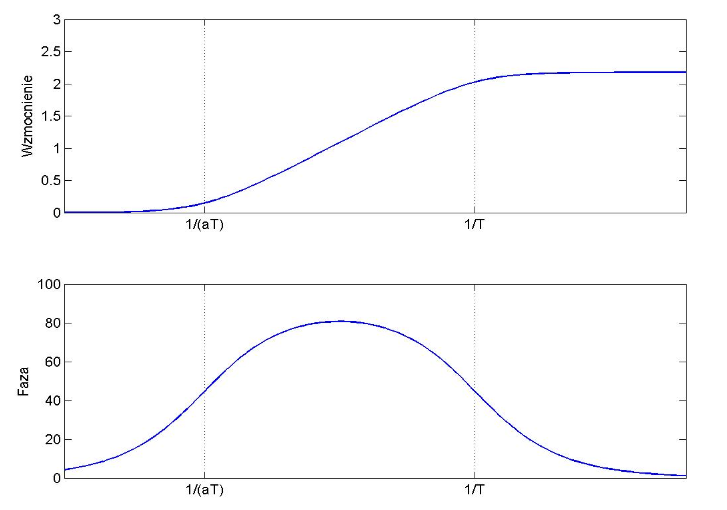
\includegraphics[width = \linewidth]{lead}
\end{frame}

\begin{frame}{Filtr górno-przepustowy}

	Maksymalna wartość fazy jest dodawana dla częstotliwości centralnej:
	\begin{equation*}
	\omega_{m} = \frac{1}{T \sqrt{a}}
	\end{equation*}
	
	Maksymalną wartość fazy można obliczyć z następującego wzoru:
	\begin{equation*}
	\sin{\phi_{m}} = \frac{a-1}{a+1}
	\end{equation*}
\end{frame}

\begin{frame}{Zera i bieguny elementu lead}
	
	
	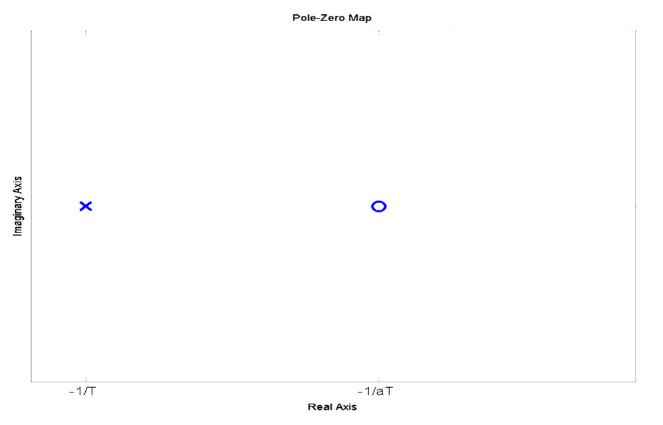
\includegraphics[width = \linewidth]{pole_lead}
	
	
\end{frame}	

% % % % % % % % % % % % % % % % % % % % % % % % % % % % % % % % % % % % % % % % % % % % % % % % % % % % % % % % % % % % %
\begin{frame}{Filtr dolno-przepustowy}

Filtr dolno-przepustowy poprawia własności układu w stanie ustalonym. Dla wysokich częstoliwości nie zmienia on własności układu (wzmocnienie jednostkowe) natomiast dla niskich częstotliwości wzmocnienie wynosi $\frac{z_1}{p_1}$ więc błąd w stanie ustalonym będzie zmniejszony o współczynnik $\frac{1}{a}$
\begin{equation*}
G_{c}(s) = \frac{1}{a} \Big(\frac{aTs + 1}{T s + 1} \Big)  \; \text{dla}\; a>1
\end{equation*}
\end{frame}

\begin{frame}{Wykres Bodego elementu typu lag}
	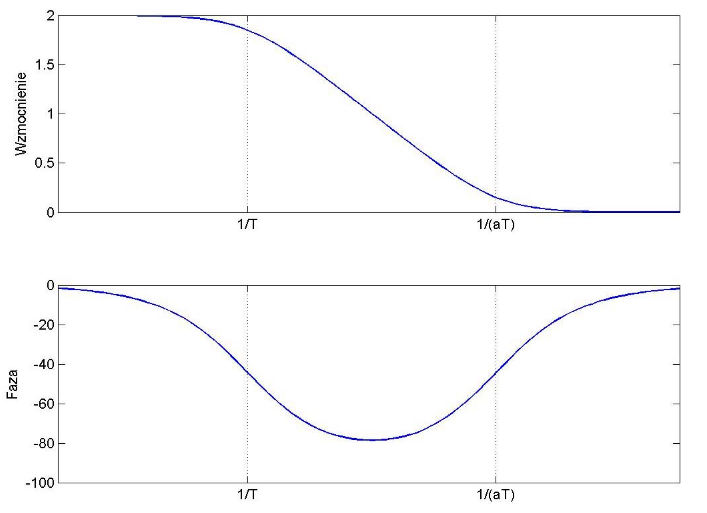
\includegraphics[width = \linewidth]{lag}
\end{frame}
\begin{frame}{Zera i bieguny elementu typu lag}

	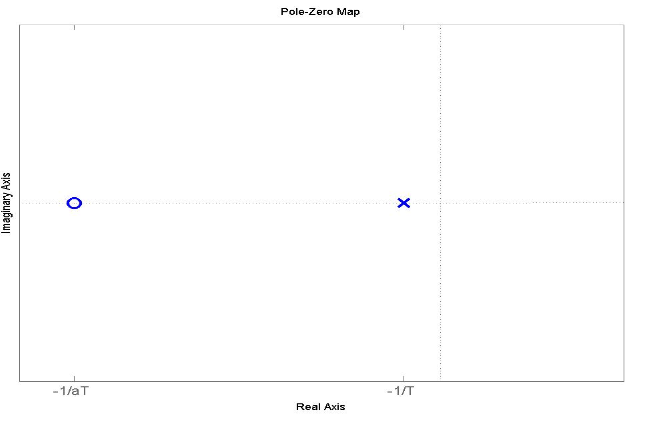
\includegraphics[width = \linewidth]{pole_lag}
\end{frame}	

\begin{frame}{Projektowanie kompensatora typu lead}

Transmitancja obiektu dla którego zaprojektowaliśmy kompensator typu lead. Z zadanym maksymalnym przeregulowaniem równym 25\%. 
	\begin{equation*}
	G = \frac{10}{s(s+1)}
	\end{equation*}

\end{frame}
	
\begin{frame}{Projektowanie kompensatora typu lead}
	\begin{equation*}
	MO = 100e^{- \frac{\xi\pi}{\sqrt{1-\xi^2}}} [\%]  
	\end{equation*}
	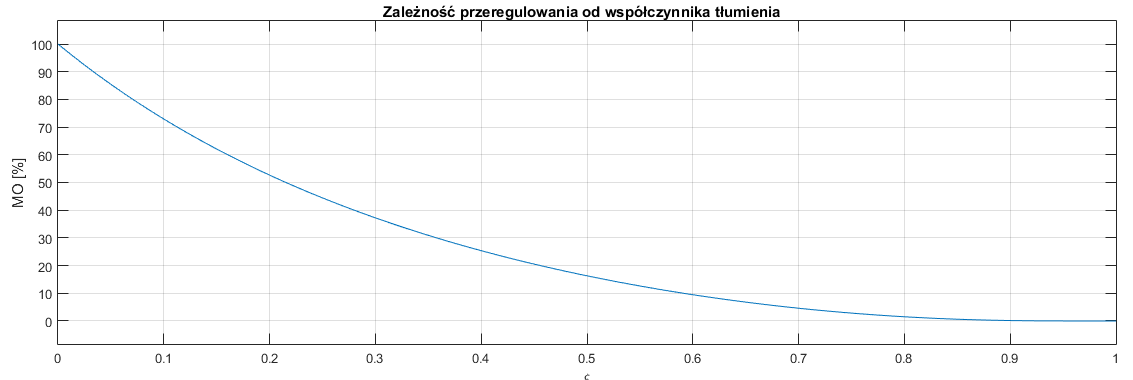
\includegraphics[width = \linewidth]{ksi}
\begin{itemize}
\item $\xi = 0.407$
\end{itemize}
\end{frame}	

\begin{frame}{Projektowanie kompensatora typu lead - zapas fazy}
	\begin{equation*}
	PM = \arctan \Bigg( \frac{2\xi}{\sqrt{\sqrt{1+4\xi^2}-2\xi^2}} \Bigg)
	\end{equation*}
	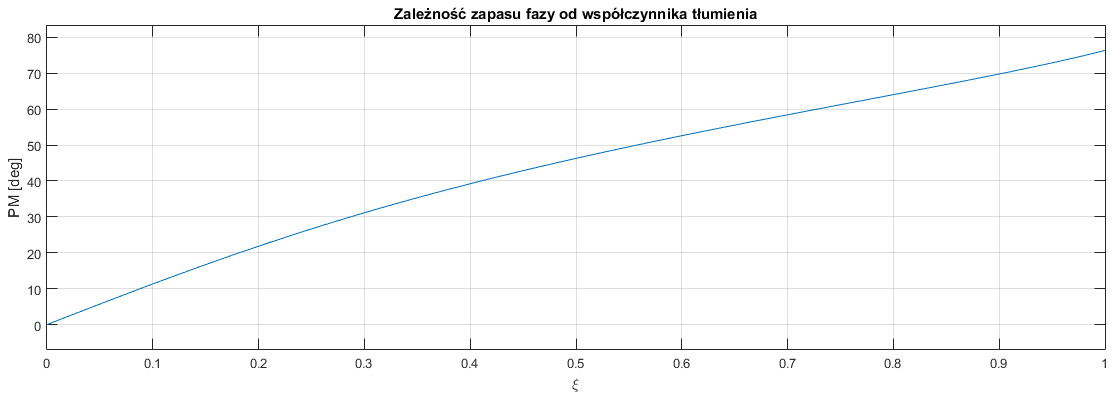
\includegraphics[width = \linewidth]{faza}

\end{frame}	
\begin{frame}{Projektowanie kompensatora typu lead}
Zapas fazy układu bez kompensacji wyznaczyliśmy za pomocą funkcji margin. Różnica zapasu fazy zadanej a obecnej w układzie bez kompensacji stanowi zapas fazy kompensatora.
	\begin{equation*}
	\phi_{m} = PM_{komp} - PM_{bez\_komp}
	\end{equation*}
Mając maksymalną wartość zapasu fazy kompensatora parametr $a$ kompensatora można wyznaczyć ze wzoru:
	\begin{equation*}
	a = \frac{1-\sin\phi_{m}}{1+sin\phi_{m}}
	\end{equation*}
Otrzymaliśmy następujące wyniki:
\begin{equation*}
\phi_{m} = 34.1 \degree
\end{equation*}
\begin{equation*}
a = 0.2815
\end{equation*}

	
\end{frame}	

\begin{frame}{Projektowanie kompensatora typu lead}
Częstotliwość $\omega_{m}$ wokół której dodawany zapas fazy kompensatora, można odczytać z wykresu Bodego układu bez kompensacji. Amplituda o wartości $-10\log(a)$ jest równa dla częstotliwości $\omega_{m}$.
\begin{equation*}
	-10\log(a) = 5.5 [dB]
 \end{equation*}
 \begin{equation*} 
 \omega_{m} = 4.28 [rad/s]
 \end{equation*}
\end{frame}


\begin{frame}{Projektowanie kompensatora typu lead}
	Ostateczne parametry kompensatora równają się:
	\begin{itemize}
		\item $a = 0.2815$
		\item $T = \frac{1}{\omega_m \sqrt{a}} = 0.4363$
	\end{itemize}
	Gdzie transmitancja wynosi:
	\begin{equation*}
	G_{c}(s) = \frac{1}{a} \bigg(\frac{s + 1/T}{s + 1/(aT)} \bigg) 
	\end{equation*}
\end{frame}

\begin{frame}[fragile]{Projektowanie kompensatora typu lead}

\begin{lstlisting} 
sys=tf(10,[1 1 0]); % system bez kompensacji
a=0.2815; % parametr a
T=0.4363; % parametr T
lead=tf([1 1/T],[alpha 1/T]); % kompensator typu LEAD

% system zamkniety po kompensacji
comp=feedback(series(sys, lead),1,-1);
% system zamkniety bez kompensacji
uncomp=feedback(sys,1,-1);

% porownanie odpowiedzi skokowych obu systemow
step(uncomp, 5)
hold on
step(comp, 5)
legend('Bez kompensacji','Po kompensacji');


\end{lstlisting}

\end{frame}

\begin{frame}{Projektowanie kompensatora typu lead}
	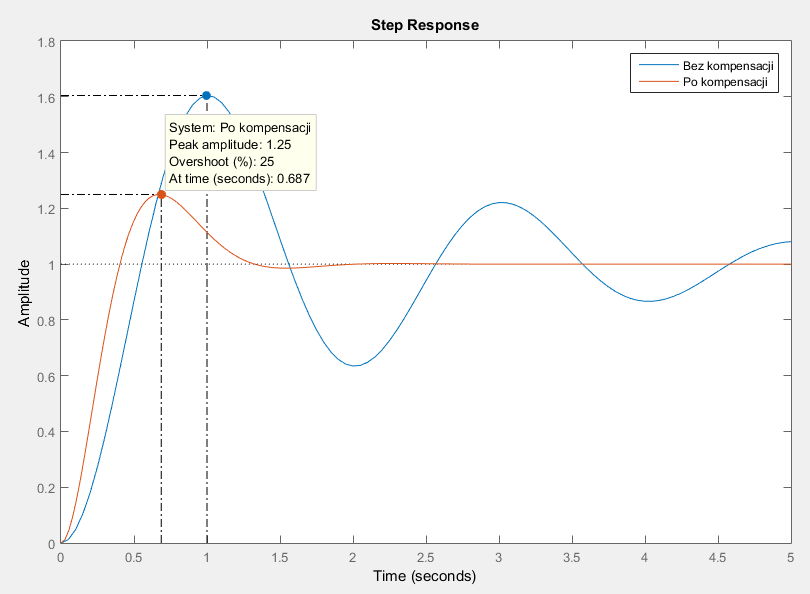
\includegraphics[width = \linewidth]{step}
\end{frame}	

\end{document}



